% !TEX encoding = UTF-8 Unicode 
\begin{filecontents*}{\jobname.xmpdata}
\Title{Opinnäytetyö}
\Author{Noora Angelva}
\end{filecontents*}

% Yllä on määritelty pdf/a-muotoon vaadittu metadata minimaalisella tavalla
%Tämän LaTeX-pohjan laadintaan ovat osallistuneet Mika Hirvensalo, Teemu Pirttimäki, Petriina Paturi ja Vesa Halava, Noora Angelva

% yksipuolinen A4
\documentclass[a4paper,12pt,oneside]{article}

\usepackage[finnish]{babel}            				
% suomenkielinen tavutus ja sanasto
\usepackage[T1]{fontenc}               				
% valitaan ääkkösfonttikoodaus
\usepackage[utf8]{inputenc}        						
% skandit utf-8 koodauksella
\usepackage{amsthm}													% theorem- yms. ympäristöt
\usepackage{amsmath}												% AMS-matematiikkatoimintoja
\usepackage{graphicx}           							
% kuvat
%\usepackage[dvips]{graphicx}           			
% ps-kuvat
\usepackage{graphicx,wrapfig,lipsum}

% Seuraavat rivit määrittävät LaTeXin oletusfontin Computer Modern sijasta käytettäväksi Arial-fontin. Poista 
% rivien ensimmäinen % jos tahdot käyttää New TX-fonttia.
%%%%%%%%%%%%%%%%%%%%%%%%%%%%%%%%%%%%%%%%%%%%%%%%
%\usepackage{newtxtext}       
%\usepackage{newtxmath}
%%%%%%%%%%%%%%%%%%%%%%%%%%%%%%%%%%%%%%%%%%%%%%%%
\usepackage[tagpdf]{axessibility} %Saavutettavuuspaketti, kaavoista tulee lukuohjelmalla luettavampia
%HUOM: LaTeXin erillinen accessibility-paketti ei toimi amsthm-paketin kanssa.
%%%%%%%%%%%%%%%%%%%%%%%%%%%%%%%%%%%%%%%%%%%%%%%%

% Seuraavat rivit määrittävät saavutettavuuden kannalta riittävän pdf/a-muodon UTUGradu-järjestelmään.
% Gradua voi olla mukavampi työstää ilman näitä, ne voi ottaa käyttöön vasta 

%%%%%%%%%%%%%%%%%%%%%%%%%%%%%%%%%%%%%%%%%%%%%%%%

\usepackage[a-3b]{pdfx}  											% Lähtökohtana pdf/a-3b
\usepackage[pdfa]{hyperref}										% pdf/a-muotoa varten


%%%%%%%%%%%%%%%%%%%%%%%%%%%%%%%%%%%%%%%%%%%%%%%%
% Testauksen vuoksi pseudolatinaa tuottava
% paketti. Et tarvitse tätä omassa työssäsi.
\usepackage{lipsum}  
%%%%%%%%%%%%%%%%%%%%%%%%%%%%%%%%%%%%%%%%%%%%%%%%
% Fontin ja tekstin määritykset

%\renewcommand{\familydefault}{\sfdefault}
%\usepackage[scaled=1]{Arial}
%\usepackage[Arial]{sfmath}
%\everymath={\sf}
\usepackage{setspace}
\usepackage{anyfontsize}
\usepackage{tabularx,lipsum}

\makeatletter
\renewcommand*\l@section{\@dottedtocline{1}{0em}{1.5em}}
\makeatother
\renewcommand{\rmdefault}{phv} % Arial
\renewcommand{\sfdefault}{phv} % Arial
\usepackage{titlesec}
\titleformat*{\subsubsection}{\normalfont}
\titleformat*{\section}{\normalfont}
\setlength{\parskip}{0pt}
\renewcommand{\baselinestretch}{1.0}
%%%%%%%%%%%%%%%%%%%%%%%%%%%%%%%%%%%%%%%%%%%%%%%%

% A4 mitat ovat 210x297 (mm), 
% ylämarginaali 30 mm, vasen marginaali 30 mm

% Lapin AMK
% 40 mm vasen reuna lapinamk
% 20 mm ylä- ja oikreuna lapinamk
% 210 - 40 - 20 = 150 leveys
% 297 - 20 -20 = 257 korkeus

%%%%%%%%%%%%%%%%%%%%%%%%%%%%%%%%%%%%%%%%%%%%%%%%
\usepackage{geometry}
\geometry{
 a4paper,
 total={150mm,257mm},
 left=40mm,
 top=20mm,
 }
%https://en.wikibooks.org/wiki/LaTeX/Page_Layout

%Suomenkieliset ympäristöt: 

\theoremstyle{plain}
\newtheorem{theorem}{Lause}
\newtheorem{lemma}{Lemma}
\newtheorem{corollary}{Seuraus}
%
\theoremstyle{definition}
\newtheorem{definition}{M\"a\"aritelm\"a}
\newtheorem{example}{Esimerkki}
%
\theoremstyle{remark}
\newtheorem{remark}{Huomautus}

%%%%%%%%%%%%%%%%%%%%%%%%%%%%%%%%%%%%%%%%%%%%%%%%
%Määrittele tässä aika, työn, kirjoittajan ja ohjaajien tiedot

\newcommand{\tekija}{{Noora Angelva}} %tekijän nimi
\newcommand{\Ohjaajat}{{Maisa Mielikäinen ja Tuija x}} %ohjaajat
\newcommand{\Toimeksiantaja}{{Yhtiö X}} %tekijän nimi
\newcommand{\titteli}{{ }} %voi jättää tyhjäksi
\newcommand{\otsikko}{{Headline}}   %Gradun otsikko
\newcommand{\tutkielma}{{Thesis}}
\newcommand{\opinnaytetyo}{{Opinäytetyö}} %Opinnatetyo
\newcommand{\aika}{{2021}}   %vuosi
\newcommand{\tutkintonimike}{{Engineer of Information and Communication Technology}}
\newcommand{\tutkintonimikeFin}{{Tieto- ja viestintätekniikan insinööri}}
\newcommand{\Koulutus}{{Engineer (Bachelor)}}
\newcommand{\KoulutusFin}{{Insinööri (AMK)}}
\newcommand{\koulutus}{{Koulutus}} %Koulutus
\newcommand{\alaotsikko}{{alaotsikko}}
\newcommand{\taustaprojekti}{{mahd. taustaprojekti}}

%%%%%%%%%%%%%%%%%%%%%%%%%%%%%%%%%%%%%%%%%%%%%%%%

%%%%%%%%%%%%%%      Dokumentin aloitus      %%%%%%%%%%%%%%%%%%

\begin{document}

%%%%%%%%%%% Kansi %%%%%%%%%%%%%%%%%%%%%%%%%%%

\pagenumbering{arabic} %sivunumerot aribialaisittain
\pagestyle{empty}  %ei sivunumeroa sivun alareunaan tälle sivulle

% Logo
\begin{center}

\includegraphics[width=6cm]{UAS_Logo}
\end{center}

% Otsikko
\vspace{8.5cm}
\begin{center}
\fontsize{16pt}{1pt}\selectfont
\otsikko \\ 
\vspace{0.7cm}
\fontsize{14pt}{1pt}\selectfont
\alaotsikko
\end{center}

% Info
\vspace{5cm}
\begin{center}
\taustaprojekti\\
\vspace{0.6cm}
\tekija \\
\vspace{0.6cm}
\opinnaytetyo \\
\koulutus\\
\tutkintonimike
\end{center}

% Vuosi
\begin{center}\fontsize{16pt}{1pt}\selectfont
\aika
\end{center}

% TIIVISTELMÄ (EN) %%%%%%%%%%%%%%%%%%%%%%%%%%%%%%%%%%%%%%%%%%%%%

\newpage\null
\pagestyle{empty}  %ei sivunumeroa sivun alareunaan

% YLATUNNISTE
\begin{minipage}{0.22\textwidth}

\includegraphics[width=3.7cm]{ylatunnisteLogo}
\end{minipage}
\begin{minipage}{0.6\textwidth}\raggedleft
Abstract of Thesis\\
\end{minipage}

\Koulutus \\
\indent\tutkintonimike \\
\rule{\textwidth}{.1mm}\\

% YLATUNNISTE END

% Tiedot
\noindent
\begin{tabularx}{\textwidth}{@{}>{\bfseries}l X@{}}
\textbf{Author} & \tekija \hspace{5cm} Year \hspace{1cm}\aika \\
\textbf{Supervisor(s)}	& \Ohjaajat \\
\textbf{Commissioned by}	& \Toimeksiantaja \\
\textbf{Subject of thesis} &	\opinnaytetyo \\
\textbf{Number of pages} &	XX + X \\
\end{tabularx}
\noindent
\rule{\textwidth}{.1mm}\\

%TIIVISTELMÄ (EN)->
\noindent
Kirjoita tähän tiivistelmä. Laita $\backslash${noindent}-komento kappaleen
alkuun, niin \LaTeX\, ei sisennä ensimmäistä riviä.

\vspace{7mm}\noindent Komento $\backslash$vspace taasen jättää sopivan välin kappaleiden väliin - 4mm näyttää aika hyvältä.

\vspace{7mm}\noindent Kirjoita tiivistelmä napakasti ja kaikenlaista toistoa välttäen.

%sivun loppuun ->
\vspace{7mm}\noindent Keywords: tiivistelmäsivu, Pro gradu -tutkielma, \LaTeX-ladontajärjestelmä.


% TIIVISTELMÄ (FIN) %%%%%%%%%%%%%%%%%%%%%%%%%%%%%%%%%%%%%%%%%

\newpage\null
\pagestyle{empty}  %ei sivunumeroa sivun alareunaan

% YLATUNNISTE
\begin{minipage}{0.22\textwidth}

\includegraphics[width=3.7cm]{ylatunnisteLogo}
\end{minipage}
\begin{minipage}{0.6\textwidth}\raggedleft
Opinnäytetyön tiivistelmä\\
\end{minipage}\

\indent\KoulutusFin \\
\indent\tutkintonimikeFin \\
\rule{\textwidth}{.1mm}\\
% YLATUNNISTE END

% Tiedot
\noindent
\begin{tabularx}{\textwidth}{@{}>{\bfseries}l X@{}}
\textbf{Tekijä} & \tekija \hspace{4cm} Vuosi \hspace{1cm}\aika \\
\textbf{Ohjaaja(t)}	& \Ohjaajat \\
\textbf{Toimeksiantaja}	& \Toimeksiantaja \\
\textbf{Tyonantaja} &	\opinnaytetyo \\
\textbf{Sivu- ja liitesivumäärä} &	XX + X \\
\end{tabularx}
\noindent\rule{\textwidth}{.1mm}\\


% TIIVISTELMä ->

\noindent Kirjoita tähän tiivistelmä. Laita $\backslash${noindent}-komento kappaleen
alkuun, niin \LaTeX\, ei sisennä ensimmäistä riviä.

\vspace{7mm}\noindent Komento $\backslash$vspace taasen jättää sopivan välin kappaleiden väliin - 4mm näyttää aika hyvältä.

\vspace{7mm}\noindent Kirjoita tiivistelmä napakasti ja kaikenlaista toistoa välttäen.

%sivun loppuun->
\vspace{7mm}\noindent Asiasanat: tiivistelmäsivu, Pro gradu -tutkielma, \LaTeX-ladontajärjestelmä.


% SISALLYSLUETTELO %%%%%%%%%%%%%%%%%%%%%%%%%%%%%%%%%%%%%%%%%

\newpage\null
\doublespacing
\tableofcontents

%Aja laTeX-käännös uudelleen saadaksesi ajantasaisen sisällysluettelon
%\cleardoublepage

%%%%%%%%%%%%%%%%%%      TEKSTI OSUUS       %%%%%%%%%%%%%%%%%
\setlength{\parskip}{12pt}
\setlength\parindent{0pt}
\renewcommand{\baselinestretch}{1.5}
%%%%%%%%%%%%%%%% Alkusanat %%%%%%%%%%%%%%%%%%%%%%%%%%%%
\newpage\null
\pagestyle{plain} 
ALKUSANAT
%\vspace{1.2cm}

Tässä luvussa kiitetään.

%%%%%%%%%%%% Kaytetyt merkit ja lyhenteet %%%%%%%%%%%5
\newpage\null
\pagestyle{plain} 
\noindent KÄYTETYT MERKIT JA LYHENTEET

%\vspace{1.2cm}
UTUGradu-järjestelmän ja PDF\LaTeX :n pdf-formaattivaatimusten takia kannattaa käyttää muita kuin eps-muotoisia kuvia. Esimerkiksi pdf-muoto käy mainiosti vektorikuville, kunhan on samaa pdf/a-3b muotoa kuin tämän tiedoston tuottama pdf-tiedosto. Parhaiten toimivat jpg-muotoiset kuvat.


%%%%%%%%%%%%%%%%    Johdanto   %%%%%%%%%%%%%%%%%%%%%%%%%%
\newpage\null
\pagestyle{plain} 

\section{JOHDANTO}

\lipsum[1]
\vspace{0.7cm}
\lipsum[1]

%%%%%%%%%%%%%%      Käsittelyosa    %%%%%%%%%%%%%%%%%%%%%%%%

\section{KÄSITTELYOSA}
\subsection{Saavutettavuus kuvateksteissä}

Kaikkiin tutkielmassa esiintyviin kuviin tulee viitata tekstissä (ks.~\ref{kuvatus1}) Lisäksi kuvatekstin tulee olla kuvaileva, koska saavutettavuuteen liittyvät alt-tekstit eivät oikein toimi käytetyn \LaTeX :n axessibility-paketin kanssa. Jos kuvan perusteella tehdään päätelmä, tulee päätelmä kuvata tekstissä. 
\begin{theorem} Oletetaan että välillä $[a,b]$ on $F'(x)=f(x)$ ja että $f$ on jatkuva.\footnote{Jatkuvuus on oleellinen seikka tässä yhteydessä.} Tällöin
\[
\int_a^bf(x)\,dx=F(b)-F(a).
\]
\end{theorem}

\subsection{Analyyttistä lukuteoriaa}

\begin{figure}[ht]
\begin{center}
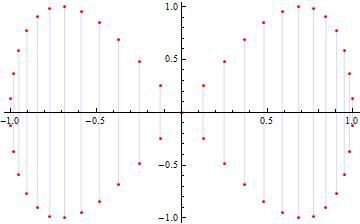
\includegraphics[width=.45\textwidth]{siivet.jpg}
\end{center}
\label{kuvatus1}
\caption{Geronon lemniskaatta välillä $[-1,1]$.}
\end{figure}

Seuraavaksi esitellään niin sanottu {\em Riemannin hypoteesi}, jonka mukaan ns. $\zeta$-funktion epätriviaalit nollakohdat sijaitsevat suoralla $\operatorname{Re}z=\frac12$.
\begin{definition} Riemannin $\zeta$-funktio määritellään sarjaesityksen \cite{Riemann}
\[
\zeta(z)=\sum_{n=1}^{\infty}\frac{1}{n^z}
\]
avulla, kun $\operatorname{Re}z>1$.
\end{definition}

\subsubsection{Matriisilaskentaa}

Nyt tarkastellaan matriisin
\[
A=\left(\begin{array}{rrr} -1 & -2 & -5\\ 3& 4& 5\\ -3 & 2 & 1 \end{array}\right)
\]
ominaisarvoja.

%%%%%%%%%%%%%%%%%%% Pohdinta %%%%%%%%%%%%%%%%%%%%%%%%%

\section{POHDINTA}
\lipsum[1]
\vspace{0.7cm}
\lipsum[1]


%%%%%%%%%%%     Lähteet     %%%%%%%%%%%%%%%%%%%%%%%%

%Kirjallisuusluettelon määrittelyssä {99} on levein kirjallisuusviitteen numero. Oikaise tarvittaessa.
\newpage\null
\section{LÄHTEET}
 
 Tässä on malli lähdeluettelosta. Luettelossa on myös hyödyllistä opinnäytekirjal-lisuutta. Mallilähdeluettelossa on kappalevälistys (ennen 0 pt, jälkeen 12 pt, rivi-väli 1), joka tulee automaattisesti, kun painaa palautusnäppäintä (Enter/Return) lähteen lopussa.  Eri lähteiden välissä ei tällöin tarvita ylimääräistä tyhjää riviä. \\

Alasuutari, P. 2007. Laadullinen tutkimus. 6. painos. Tampere: Vastapaino.





%%%%%%%%%%% liitteet %%%%%%%%%%%%%%%%%%%%%%%%%
\newpage\null
\section{LIITTEET}

Tässä luvussa esitetään niin kutsuttu Newtonin-Leibnizin kaava Liitteistä tehdään liiteluettelo, joka on omalla sivulla ennen varsinaisia liitesivuja. Liitteet on numeroimaton otsikko ja merkitään sisällykseen ja tekstiin näin: LIIT-TEET. Liitteet luetellaan ja otsikoidaan esiintymisjärjestyksessä seuraavan mal-lin mukaisesti: \\

Liite 1. 	Aalto, internet-osoite\\
Liite 2. 	Aalto, valokuva\\
Liite 3. 	Aalto, kokeilu 1\\
Liite 4. 	Aalto, kokeilu 2\\


\end{document}
